\documentclass{article}
\usepackage[utf8]{inputenc}
\usepackage[T1]{fontenc}
\usepackage[spanish]{babel}
\usepackage{hyperref}
\usepackage{url}
\usepackage{booktabs}
\usepackage{amsfonts}
\usepackage{amsmath}
\usepackage{nicefrac}
\usepackage{microtype}
\usepackage{graphicx}
\usepackage{caption}
\usepackage{listings}
\usepackage{color}
\graphicspath{{./images/}}
\usepackage{lmodern}  % Latin Modern, versión escalable de Computer Modern
\usepackage[margin=2.5cm]{geometry}

\title{Trabajo Práctico 1.1 -- Simulación}
\author{
    Renzo Aimaretti \\ \texttt{renzoceronueve@gmail.com}
    \and
    Facundo Sosa Bianciotto \\ \texttt{facundososabianciotto@gmail.com}
    \and
    Vittorio Maragliano \\ \texttt{maraglianovittorio@gmail.com}
    \and
    Ignacio Amelio Ortiz \\ \texttt{nameliortiz@gmail.com}
    \and
    Nicolás Roberto Escobar \\ \texttt{escobar.nicolas.isifrro@gmail.com}
    \and
    Juan Manuel De Elia \\ \texttt{juanmadeelia@gmail.com}
}

\begin{document}
\maketitle

\begin{abstract}
Este informe presenta el desarrollo e implementación de una simulación computacional del funcionamiento de una ruleta, como introducción a los conceptos básicos de la materia Simulación. El modelo fue implementado en Python 3 e incluye generación de números aleatorios, estructuras de datos, análisis estadístico y visualización de resultados mediante gráficos. Se realizaron múltiples corridas del experimento para analizar el comportamiento probabilístico del sistema, contrastar los resultados con las expectativas teóricas y evaluar la aleatoriedad y el sesgo del modelo. El objetivo principal es familiarizarse con herramientas y conceptos esenciales de simulación estocástica aplicados a un sistema simple y ampliamente conocido.
\end{abstract}

\section{Introducción}
En el marco de la cátedra Simulación, este trabajo tiene como objetivo desarrollar una primera aproximación al estudio de sistemas aleatorios mediante la construcción e implementación de un modelo simple: una ruleta. A través de este ejemplo clásico de juego de azar, se busca comprender cómo se puede simular el comportamiento de un sistema estocástico utilizando programación.

Se simulará la corrida de una ruleta tipo europea, compuesta por 37 números (del 0 al 36), replicando el proceso de selección aleatoria que ocurre en cada giro. El modelo permitirá definir distintos parámetros de entrada, como la cantidad de tiradas o el número apostado, y generará datos que serán analizados estadísticamente.

Durante el desarrollo se emplearán herramientas del lenguaje Python 3.x, incluyendo funciones de generación de números aleatorios, estructuras de control, listas, y bibliotecas para visualización como \texttt{Matplotlib}. Además, se calcularán frecuencias absolutas y relativas, y se compararán los resultados obtenidos con los valores esperados desde un enfoque probabilístico.

Este trabajo busca practicar conceptos teóricos y aplicar herramientas computacionales para analizar el comportamiento de un sistema sencillo, sentando las bases para simulaciones más complejas en trabajos futuros.

\section{Descripción del programa}
\subsection{Funciones del programa}
El programa está compuesto por cuatro funciones principales que permiten la simulación, cálculo de estadísticas, visualización de resultados y la ejecución principal. A continuación, se describe cada una de ellas en detalle.

\subsection{Conceptos teóricos utilizados}
Se emplearon las siguientes formulas de estadistica:

1. Varianza esperada:
\[
\text{Var}(X) = \frac{(b - a)^2}{12}
\]

2. Varianza muestral:
\[
s^2 = \frac{1}{n-1} \sum_{i=1}^{n} (x_i - \bar{x})^2
\]

3. Desviación estándar real:
\[
\sigma_{\text{real}} = \sqrt{\frac{1}{n-1} \sum_{i=1}^{n} (x_i - \bar{x})^2}
\]

4. Desviación estándar esperada:
\[
\sigma = \frac{b - a}{\sqrt{12}}
\]

5. Frecuencia relativa esperada:
\[
f_{\text{esp}} = \frac{n_{\text{esp}}}{n_{\text{total}}}
\]
donde \( n_{\text{esp}} \) es la frecuencia esperada y \( n_{\text{total}} \) es el total de observaciones.

6. Frecuencia relativa real:
\[
f_{\text{real}} = \frac{n_{\text{real}}}{n_{\text{total}}}
\]
donde \( n_{\text{real}} \) es la frecuencia observada y \( n_{\text{total}} \) es el total de observaciones.

7. Promedio esperado:
\[
\mu_{\text{esp}} = E[X] = \sum_{i=1}^{n} p_i \cdot x_i
\]
donde \( p_i \) es la probabilidad de que ocurra el evento \( i \) y \( x_i \) es el valor correspondiente a ese evento.

8. Promedio real:
\[
\mu_{\text{real}} = \frac{1}{n} \sum_{i=1}^{n} x_i
\]
donde \( x_i \) son las observaciones reales.

\subsubsection{simular\_ruleta}
La función \texttt{simular\_ruleta} es la encargada de generar las tiradas aleatorias de la ruleta según la cantidad solicitada:

\begin{verbatim}
def simular_ruleta(tiradas):
    numeros_sorteados = []
    for _ in range(tiradas):
        resultado = random.randint(0, 36)
        numeros_sorteados.append(resultado)
    return numeros_sorteados
\end{verbatim}

Esta función toma como único parámetro \texttt{tiradas}, que representa la cantidad de veces que se lanzará la ruleta. Para cada tirada, genera un número pseudoaleatorio entre 0 y 36 (simulando una ruleta europea) utilizando la función \texttt{random.randint()}. Todos los resultados se almacenan en una lista que es retornada al finalizar la ejecución.

\subsubsection{calcular\_estadisticas}
Esta función procesa los resultados de las tiradas y calcula diferentes métricas estadísticas:

\begin{verbatim}
def calcular_estadisticas(numeros_sorteados, numero_elegido):
    frecuencia_relativa = []
    promedio = []
    desviacion = []
    varianza = []

    conteo = 0
    suma = 0

    for i in range(1, len(numeros_sorteados) + 1):
        tirada = numeros_sorteados[i - 1]
        suma += tirada
        if tirada == numero_elegido:
            conteo += 1

        fr = conteo / i
        prom = suma / i
        
        frecuencia_relativa.append(fr)
        promedio.append(prom)
        
        if i > 1:
            var = sum((numeros_sorteados[j-1] - prom) ** 2 
                for j in range(i)) / (i - 1)
            desv = math.sqrt(var)
        else:
            var = 0
            desv = 0
            
        desviacion.append(desv)
        varianza.append(var)

    return frecuencia_relativa, promedio, desviacion, varianza
\end{verbatim}

Recibe como parámetros:
\begin{itemize}
    \item \texttt{numeros\_sorteados}: Lista con los resultados de cada tirada.
    \item \texttt{numero\_elegido}: Número específico para calcular su frecuencia relativa.
\end{itemize}

Para cada tirada calcula:
\begin{itemize}
    \item \textbf{Frecuencia relativa}: Proporción de veces que aparece el número elegido.
    \item \textbf{Promedio}: Media aritmética de todos los valores sorteados hasta el momento.
    \item \textbf{Varianza}: Dispersión de los valores respecto a la media, usando la fórmula de varianza muestral.
    \item \textbf{Desviación estándar}: Raíz cuadrada de la varianza.
\end{itemize}

Cada cálculo se realiza de forma acumulativa, almacenando los resultados para cada número de tiradas desde 1 hasta el total.

\subsubsection{graficar}
Esta función se encarga de generar y guardar los gráficos de las estadísticas calculadas:

\begin{verbatim}
def graficar(x, y, valor_esperado, titulo, ylabel, nombre_archivo):
    plt.figure()
    plt.plot(x, y, label="Simulado", color='red')
    plt.axhline(y=valor_esperado, color='blue', 
                linestyle='--', label="Esperado")
    plt.xlabel("n (número de tiradas)")
    plt.ylabel(ylabel)
    plt.title(titulo)
    plt.legend()
    plt.grid(True)
    plt.savefig(nombre_archivo)
    plt.close()
\end{verbatim}

Recibe como parámetros:
\begin{itemize}
    \item \texttt{x}: Eje x (número de tiradas).
    \item \texttt{y}: Datos a graficar.
    \item \texttt{valor\_esperado}: Valor teórico esperado.
    \item \texttt{titulo}: Título del gráfico.
    \item \texttt{ylabel}: Etiqueta del eje y.
    \item \texttt{nombre\_archivo}: Nombre del archivo donde se guardará el gráfico.
\end{itemize}

Genera un gráfico que muestra la evolución de la estadística calculada a medida que aumenta el número de tiradas, comparándola con el valor teórico esperado.

\subsubsection{main}
La función principal coordina la ejecución del programa:

\begin{verbatim}
  def main():
  # La varianza de que un numero X salga en la ruleta sigue una ditribucion uniforme 
  varianzaEsperada = ((37**2)-1)/12
  desvioEsperado = math.sqrt(varianzaEsperada)
  parser = argparse.ArgumentParser()
  parser.add_argument("-c", "--corridas", type=int, default=1, help="Número de corridas")
  parser.add_argument("-n", "--tiradas", type=int, default=1000, help="Número de tiradas por corrida")
  parser.add_argument("-e", "--elegido", type=int, default=17, help="Número elegido")
  args = parser.parse_args()

  corridas = args.corridas
  tiradas = args.tiradas
  numero_elegido = args.elegido

  numeros = simular_ruleta(tiradas)
  frn, vpn, vd, vv = calcular_estadisticas(numeros, numero_elegido)
  x = list(range(1, tiradas + 1))
  graficar(x, frn, 1 / 37, f"Una sola corrida - Frecuencia relativa del número {numero_elegido}", 
  "Frecuencia relativa", f"grafica_frecuencia.png")
  graficar(x, vpn, 18, f"Una sola corrida  - Valor promedio de las tiradas", "Valor promedio",
   f"grafica_promedio.png")
  graficar(x, vd, desvioEsperado, f"Una sola corrida  - Desvío respecto al valor esperado",
  "Desvío", f"grafica_desvio.png")
  graficar(x,vv, varianzaEsperada, f"Una sola corrida  - Varianza respecto al valor esperado",
   "Varianza", f"grafica_varianza")

  print("Simulación finalizada. Gráficos guardados.")

  # Preparar listas para almacenar resultados de todas las corridas
  todas_frn = []
  todas_vpn = []
  todos_vd = []
  todos_vv = []
  
  # Realizar todas las corridas y almacenar resultados
  for i in range(corridas):
      numeros = simular_ruleta(tiradas)
      frn, vpn, vd, vv = calcular_estadisticas(numeros, numero_elegido)
      todas_frn.append(frn)
      todas_vpn.append(vpn)
      todos_vd.append(vd)
      todos_vv.append(vv)
  
  x = list(range(1, tiradas + 1))
  
  # Crear gráficas con todas las corridas superpuestas
  plt.figure(figsize=(10, 6))
  for i, frn in enumerate(todas_frn):
      plt.plot(x, frn, label=f"Corrida {i+1}", alpha=0.7)
  plt.axhline(y=1/37, color='black', linestyle='--', label="Esperado")
  plt.xlabel("n (número de tiradas)")
  plt.ylabel("Frecuencia relativa")
  plt.title(f"Frecuencia relativa del número {numero_elegido} - {corridas} corridas")
  plt.legend()
  plt.grid(True)
  plt.savefig("grafica_frecuencia_todas.png")
  plt.close()
  
  plt.figure(figsize=(10, 6))
  for i, vpn in enumerate(todas_vpn):
      plt.plot(x, vpn, label=f"Corrida {i+1}", alpha=0.7)
  plt.axhline(y=18, color='black', linestyle='--', label="Esperado")
  plt.xlabel("n (número de tiradas)")
  plt.ylabel("Valor promedio")
  plt.title(f"Valor promedio de las tiradas - {corridas} corridas")
  plt.legend()
  plt.grid(True)
  plt.savefig("grafica_promedio_todas.png")
  plt.close()
  
  plt.figure(figsize=(10, 6))
  for i, vd in enumerate(todos_vd):
      plt.plot(x, vd, label=f"Corrida {i+1}", alpha=0.7)
  plt.axhline(y=desvioEsperado, color='black', linestyle='--', label="Esperado")
  plt.xlabel("n (número de tiradas)")
  plt.ylabel("Desvío")
  plt.title(f"Desvío respecto al valor esperado - {corridas} corridas")
  plt.legend()
  plt.grid(True)
  plt.savefig("grafica_desvio_todas.png")
  plt.close()
  
  plt.figure(figsize=(10, 6))
  for i, vv in enumerate(todos_vv):
      plt.plot(x, vv, label=f"Corrida {i+1}", alpha=0.7)
  plt.axhline(y=varianzaEsperada, color='black', linestyle='--', label="Esperado")
  plt.xlabel("n (número de tiradas)")
  plt.ylabel("Varianza")
  plt.title(f"Varianza respecto al valor esperado - {corridas} corridas")
  plt.legend()
  plt.grid(True)
  plt.savefig("grafica_varianza_todas.png")
  plt.close()
\end{verbatim}

Esta función:
\begin{itemize}
    \item Calcula los valores teóricos esperados para la varianza ($(37^2-1)/12$) y el desvío estándar.
    \item Procesa los argumentos de línea de comandos.
    \item Ejecuta la simulación para una corrida y genera los gráficos individuales.
    \item Realiza múltiples corridas y genera gráficos comparativos.
\end{itemize}

Los valores teóricos utilizados son:
\begin{itemize}
    \item Frecuencia relativa esperada: $1/37$ (probabilidad de que salga cualquier número específico)
    \item Promedio esperado: $18$ (valor medio de los números de la ruleta)
    \item Varianza esperada: $((37^2-1)/12) \approx 114.67$ (fórmula para distribución uniforme discreta)
    \item Desvío estándar esperado: $\sqrt{varianza} \approx 10.71$
\end{itemize}
\section{Graficas}
El programa genera dos conjuntos de gráficas:

\subsection{Gráficas individuales}
Para una sola corrida, se generan cuatro gráficas que muestran:
\subsubsection{Frecuencia relativa del número elegido}
Muestra cómo evoluciona la proporción de veces que aparece el número elegido, comparada con el valor teórico de $1/37 \approx 0.027$.
\begin{figure}
  \centering
  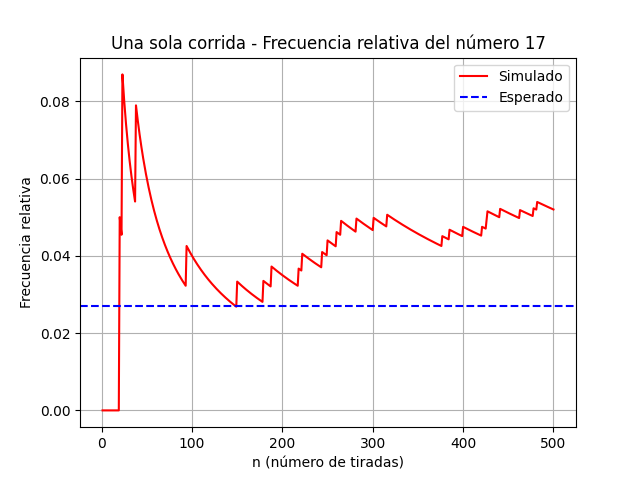
\includegraphics[width=0.8\textwidth]{grafica_frecuencia.png}
  \caption{Frecuencia relativa del número elegido a medida que aumenta el número de tiradas}
  \label{fig:frecuencia_relativa}
\end{figure}

\subsubsection{Valor promedio de las tiradas}
Muestra la evolución del promedio de los números sorteados, comparado con el valor teórico esperado de 18.
\begin{figure}
  \centering
  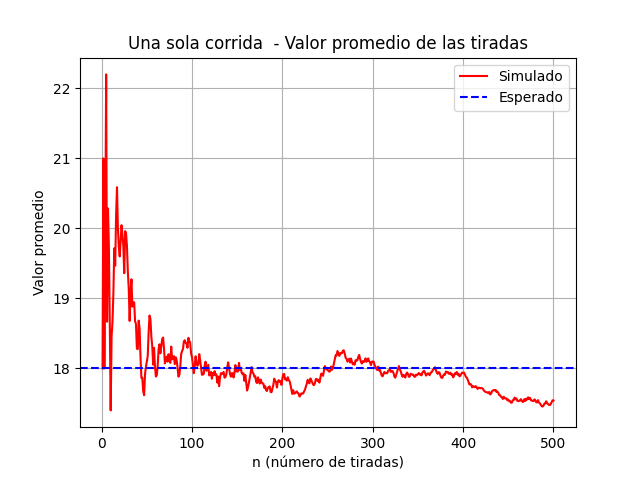
\includegraphics[width=0.8\textwidth]{grafica_promedio.png}
  \caption{Valor promedio de las tiradas a medida que aumenta el número de tiradas}
  \label{fig:promedio_individual}
\end{figure}

\subsubsection{Desvío estándar}
Muestra cómo evoluciona el desvío estándar de los valores, comparado con el desvío teórico esperado de $\sqrt{((37^2-1)/12)} \approx 10.71$.
\begin{figure}
  \centering
  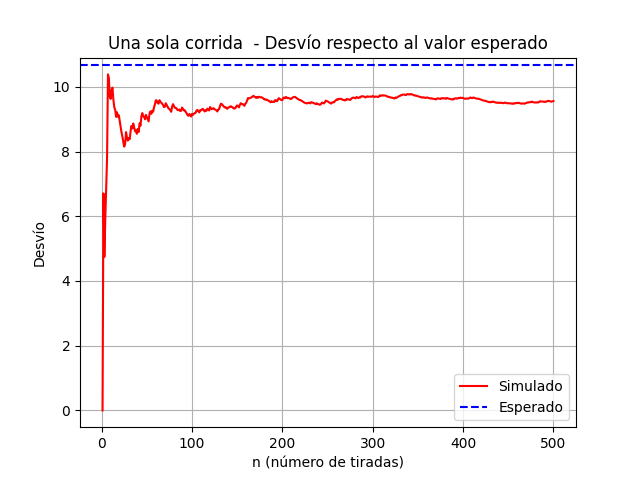
\includegraphics[width=0.8\textwidth]{grafica_desvio.png}
  \caption{Desvío estándar a medida que aumenta el número de tiradas}
  \label{fig:desvio_individual}
\end{figure}

\subsubsection{Varianza}
Muestra la evolución de la varianza, comparada con el valor teórico esperado de $((37^2-1)/12) \approx 114.67$.
\begin{figure}
  \centering
  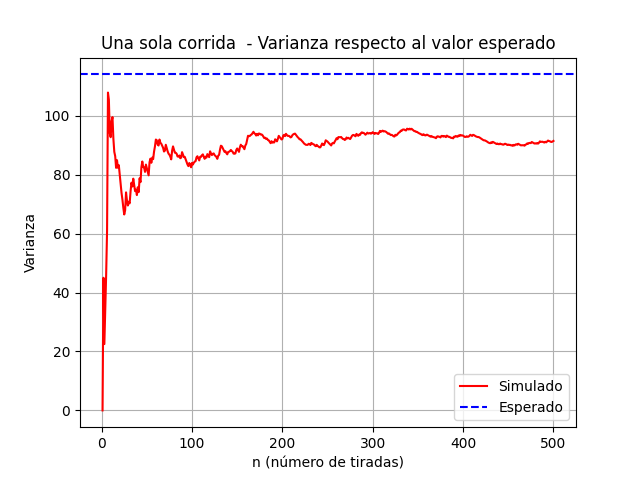
\includegraphics[width=0.8\textwidth]{grafica_varianza.png}
  \caption{Varianza a medida que aumenta el número de tiradas}
  \label{fig:varianza_individual}
\end{figure}

\subsection{Gráficas comparativas}
Para múltiples corridas, se generan gráficas que superponen los resultados de todas las corridas para cada estadística, permitiendo observar la variabilidad entre diferentes ejecuciones de la simulación.

\subsubsection{Frecuencia relativa comparativa}
\begin{figure}
  \centering
  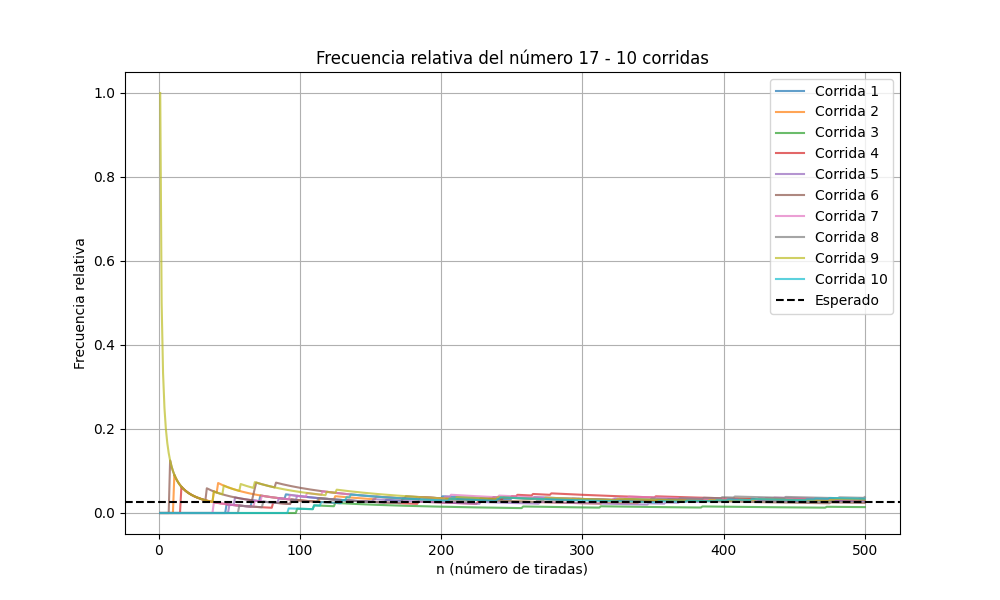
\includegraphics[width=0.8\textwidth]{grafica_frecuencia_todas.png}
  \caption{Frecuencia relativa del número elegido para múltiples corridas}
  \label{fig:frecuencia}
\end{figure}

\subsubsection{Valor promedio comparativo}
\begin{figure}
  \centering
  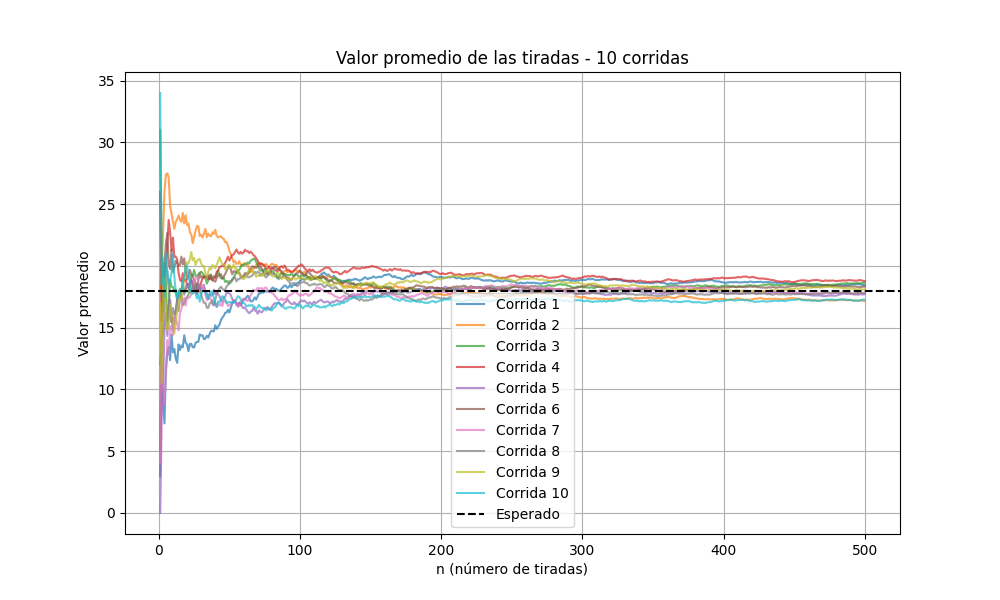
\includegraphics[width=0.8\textwidth]{grafica_promedio_todas.png}
  \caption{Valor promedio de las tiradas para múltiples corridas}
  \label{fig:promedio}
\end{figure}

\subsubsection{Desvío estándar comparativo}
\begin{figure}
  \centering
  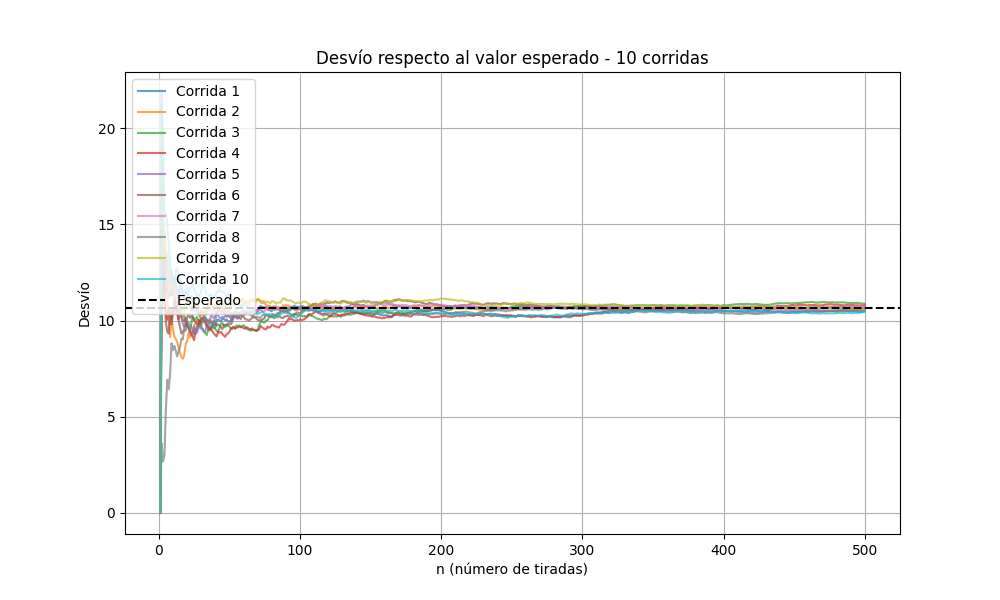
\includegraphics[width=0.8\textwidth]{grafica_desvio_todas.png}
  \caption{Desvío estándar para múltiples corridas}
  \label{fig:desvio}
\end{figure}

\subsubsection{Varianza comparativa}
\begin{figure}
  \centering
  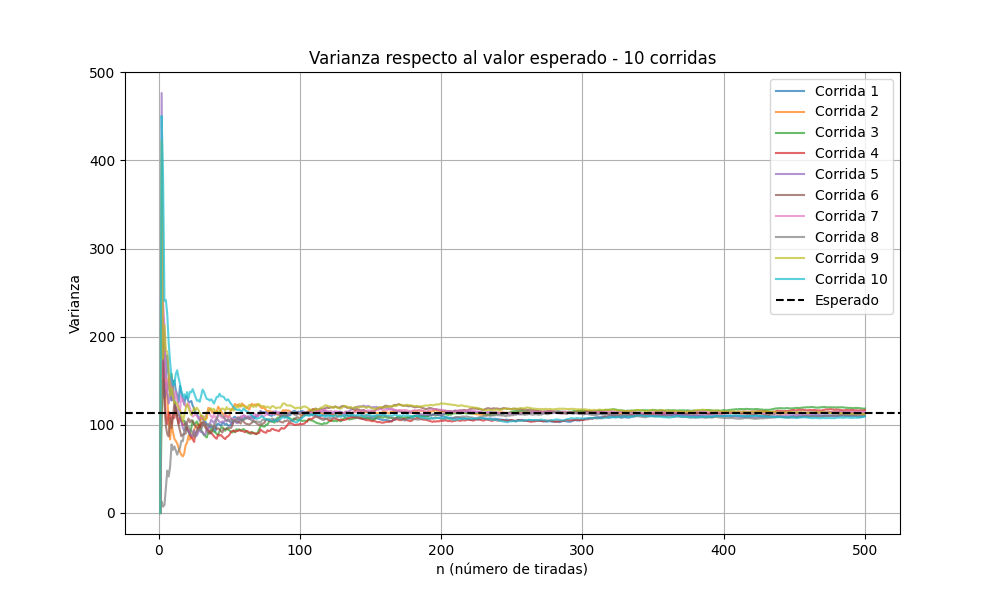
\includegraphics[width=0.8\textwidth]{grafica_varianza_todas.png}
  \caption{Varianza para múltiples corridas}
  \label{fig:varianza}
\end{figure}

En estas gráficas podemos observar cómo, a medida que aumenta el número de tiradas, los valores calculados tienden a acercarse a los valores teóricos esperados, demostrando la ley de los grandes números. También se aprecia la variabilidad entre diferentes corridas, que disminuye con el aumento del número de tiradas.
\section{Conclusiones}
A partir de la simulación realizada y el análisis de los resultados obtenidos, podemos extraer las siguientes conclusiones:

\begin{itemize}
    \item La simulación computacional de la ruleta produce resultados que concuerdan con los valores teóricos esperados cuando el número de tiradas es suficientemente grande, verificando la Ley de los Grandes Números.
    
    \item La frecuencia relativa de aparición de un número específico converge al valor teórico de $1/37 \approx 0.027$, aunque presenta fluctuaciones significativas con pocas tiradas.
    
    \item El valor promedio de los números sorteados tiende a estabilizarse alrededor del valor teórico de 18, que es el valor medio de una distribución uniforme entre 0 y 36.
    
    \item La varianza muestral converge al valor teórico de $((37^2-1)/12) \approx 114.67$, que corresponde a la varianza de una distribución uniforme discreta.
    
    \item La realización de múltiples corridas permite apreciar la variabilidad inherente al proceso aleatorio y cómo esta variabilidad disminuye con el aumento del número de tiradas.
    
    \item Las herramientas utilizadas (Python, Matplotlib) resultaron adecuadas para la simulación y visualización de los resultados, permitiendo un análisis claro de los fenómenos estadísticos involucrados.
\end{itemize}

Esta simulación simple constituye una primera aproximación al estudio de sistemas estocásticos, sentando las bases metodológicas para el análisis de sistemas más complejos en el futuro.
\end{document}